
\chapter{JTWPA characterization}
\label{c:twpa_exp}

The experimental results presented in this chapter correspond to the sixth JTWPA design revision.  For reasons that remain largely unknown, the first few generations of devices suffered from large insertion losses that prevented the demonstration of compelling amplifier performance.  Some of these results appear in reference \cite{slichterthesis}.  The fourth through sixth design revisions were fabricated at MIT-Lincoln Labs (LL), and resulted in generally better device performance.  These devices were primarily designed at QNL, though the professional mask layout team at LL did much of the layout in generations five and six using automated scripts, permitting mask design revisions to be made much more easily.  The sixth generation design revision was the first to incorporate RPM loading structures, in concert with the development of the dispersion engineering theory in 2014.  Many, many measurements were conducted over the entire course of the development of the JTWPA; from measurement records, the experiments on generations four, five, and six comprised seven, 23, and 30 dilution refrigerator cycles, respectively, in the period from August 28, 2012 through the final cooldown for generation six on January 1, 2015.

\section{Device fabrication}\label{s:twpa_fab}

\begin{figure*}
\begin{center}
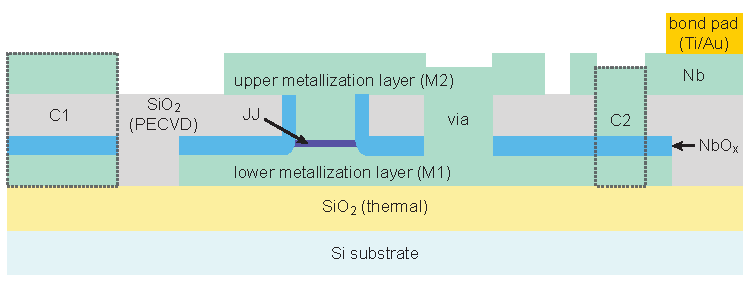
\includegraphics[width=5in]{twpa_exp/DSM_stackup.pdf}
\end{center}
\caption[Deep submicron process layers]{Schematic of the DSM process layers.  Metal layers are 150 nm thick, the PECVD layer is 200 nm thick, and the NbO$_x$ layer is 50 nm thick.  Schematic is not shown to scale.}
\label{fig:DSM_stackup}
\end{figure*}

The RPM-JTWPA is a fairly complex device, requiring the precision fabrication of five lumped-element components per unit cell of the device, and about 2000 unit cells are required to achieve enough gain to approach quantum-limited system noise.  For high-quality amplifier operation, these components should have a high degree of uniformity, requiring tight controls and process tests.  The foundry at LL is quite sophisticated, with extensive process controls including a test suite of co-fabricated structures to characterize the process performance across an entire 200 mm wafer.  The JTWPA is fabricated in the deep submicron (DSM) process, primarily used for manufacturing rapid single flux quantum (RSFQ) superconducting digital electronics, with many thousands of junctions per chip.  For a very complete description of this process, see reference \cite{Tolpygo2014}.  A schematic of the metalization and dielectric layers in DSM is shown in Fig. \ref{fig:DSM_stackup}. DSM is a fully planarized Nb/Al-AlOx/Nb trilayer process fabricated on 200 mm wafers using a modern, CMOS compatible toolset. Process modules include 248 nm photolithography, anodization, high-density plasma etching, PVD metal deposition, PECVD SiOx deposition, and chemical mechanical polishing.

Devices are fabricated on a 750 $\mu$m silicon substrate (pale blue) with a 500 nm layer of thermal SiO$_2$ (pale yellow).  Josephson junctions are defined using 248 nm optical lithography (stepper, 5x reduction) and subtractive dry etching of the Nb/Al-AlOx/Nb trilayer; the Al-AlOx is shown as a thin dark purple stripe.    Anodization of the lower Nb layer forms a thin NbO$_x$ protective layer around the junction (blue).  The inter-layer dielectric is a low-temperature PECVD silicon oxide (light gray).  The lower and upper Nb wiring layers are shown in pale green (M1 and M2, respectively); electrical connections between the layers are formed using vias (center-right).   Parallel-plate capacitors are formed implicitly where the upper and lower metallization layers overlap due to the intermediate PECVD and NbO$_x$ layers (C1, shown at left and outlined in a dashed line).  An additional high-capacitance structure can be formed by creating a via from the upper metallization layer to the anodization layer (C2, shown at right and outlined in a dashed line); C2 provides a specific capacitance approximately 35 times larger than C1.  Electrical contact is made to the chip through titanium/gold bond pads (yellow).

\begin{figure*}
\begin{center}
\includegraphics[width=4in]{twpa_exp/chip_false_color.pdf}
\end{center}
\caption[RPM JTWPA false-color optical micrograph]{False-color optical micrograph of chip layout.  M1 is shown as gray, with cutouts to form islands and accommodate the meander inductor.  JJs are drawn in light blue.  The top plate of the capacitance to ground is formed from M2 and colored yellow.  The coupling capacitance to the resonator is formed from C1; the top plate (M2 layer) is colored purple.  The resonator capacitance is formed from C2; the top plate (M2 layer) is colored green.  The resonator meander inductor is colored orange; the via from M2 to M1 is the wider square at the bottom of the trace.  The spacing between Josephson junctions is 16 $\mu$m.}
\label{fig:chip}
\end{figure*}

A false-color optical micrograph of about 10 unit cells is shown in Fig. \ref{fig:chip}.  The ground plane of the JTWPA is formed from M1.  The primary trace forming the transmission line itself is formed from M2, utilizing C1 for capacitance to ground.  A small ground plane cutout surrounds an M1 island, accommodating the Josephson junction and a via back up to M2.  The dispersion-modifying resonators are capacitively coupled to this island through C1.  A meander inductor is formed from M2 inside a ground plane cutout and is electrically connected to ground at the end with a via.  The capacitance for the resonator is formed from C2.

\begin{figure*}
\begin{center}
\includegraphics[width=4.6in]{twpa_exp/chip_pic.png}
\end{center}
\caption[RPM JTWPA chip photograph]{Macro photograph of a 2037 JJ RPM JTWPA.  The chip is 5 mm $\times$ 5 mm.}
\label{fig:chip_pic}
\end{figure*}

We use process monitor structures distributed across the 200 mm wafer to determine the junction critical current density $J_c = 5.8$ $\mu$A/$\mu$m$^2$ and junction specific capacitance $C_s = 70$ fF/$\mu$m$^2$.  The particular JTWPA device which is the main subject of this chapter features 1 $\mu$m diameter junctions with critical current $I_0 = 4.6$ $\mu$A, intrinsic junction capacitance $C_J = 55$ fF, and an external capacitance to ground $C = 45$ fF shunting the junction.  The critical current density was somewhat higher than designed, resulting in a small-signal impedance of 40 $\Omega$. When the JTWPA is pumped, the effective Josephson inductance increases, resulting in a small increase in impedance of approximately 2 $\Omega$. A better match to 50 $\Omega$ has been measured in similar devices with critical current densities closer to the target parameters.  A photograph of a 2037 junction device is shown in Figure \ref{fig:chip_pic}.

\begin{figure*}
\begin{center}
\includegraphics[width=6in]{twpa_exp/masks.png}
\end{center}
\caption[Example JTWPA layout masks]{\textbf{a} Chip layout for 50 $\Omega$ 5022 JJ non-RPM device, from Reticle A. \textbf{b} Close-up of \textbf{a}, showing CPW-to-microstrip transition and nonlinear transmission line segment. \textbf{c} Chip layout for 50 $\Omega$, 2037 JJ RPM device with 20 fF coupling capacitors, from Reticle B. \textbf{d} Close-up of \textbf{c}.}
\label{fig:masks}
\end{figure*}

Several other device designs were co-fabricated along with the particular chip design which is the subject of the bulk of the results in this chapter.  All in all, two full reticles were used for generation six, providing 13 individual chip designs in each reticle with 3 chips of process test structures.  Reticle A was dedicated to JTWPAs without RPM resonators, as these devices were known to work well.  Reticle B was dedicated to JTWPAs with the very first attempt at RPM loading, which turned out to work quite well and produce the first JTWPAs with significant gain and nearly quantum-limited noise.  Various images of the mask layouts from generation six are shown in Figure \ref{fig:masks}.

\subsection{Loss tangent extraction}

\begin{figure*}
\begin{center}
\includegraphics[width=6in]{twpa_exp/test_res.png}
\end{center}
\caption[Test resonator masks]{\textbf{a} Chip layout for C2 layer test resonators.  \textbf{b} Close-up of the low-coupling, high-impedance test resonator from the left side of \textbf{a}.}
\label{fig:test_res}
\end{figure*}

The loss tangents of the C1 and C2 capacitors were determined by measuring the internal quality factor of lumped-element test resonators.  The chip layout for the C2 capacitor test resonators is shown in Figure \ref{fig:test_res}a.  The equivalent structures for measuring the C1 layer are similar, though the capacitors have a much smaller footprint due to the larger specific capacitance.  The resonators are a differential design but are normally measured in a CPW launch with one side of the resonator wirebonded to ground.  Due to the differential design, the two capacitors which form $C$ combine in series, thus the total capacitance is half that of each physical capacitor.  The resonators are all targeted at the same nominal frequency, but with two impedance variations and two coupling strength variations.

The total inductance $L$ of the structure is purely geometric, and can be accurately predicted using finite-element simulation tools.  The coupling capacitance $C_c$ is designed to be very small compared to the resonator inductance $C$ so as to avoid loading the resonant frequency.  Furthermore, $C_c$ is designed as an interdigital capacitor, which generally has a much higher intrinsic quality factor than the overlap capacitors formed by C1 and C2, and thus should not effect the total coupling strength.  Therefore, measuring the resonant frequency of the test resonators calibrates the specific capacitance for the capacitor layer under consideration, while extracting the internal quality factor $Q_i$ provides the loss tangent of the capacitor layer.  For details on the algorithm used to extract $Q_i$ from a reflection measurement, see Appendix D of reference \cite{Weber2014a}.

\begin{figure*}
\begin{center}
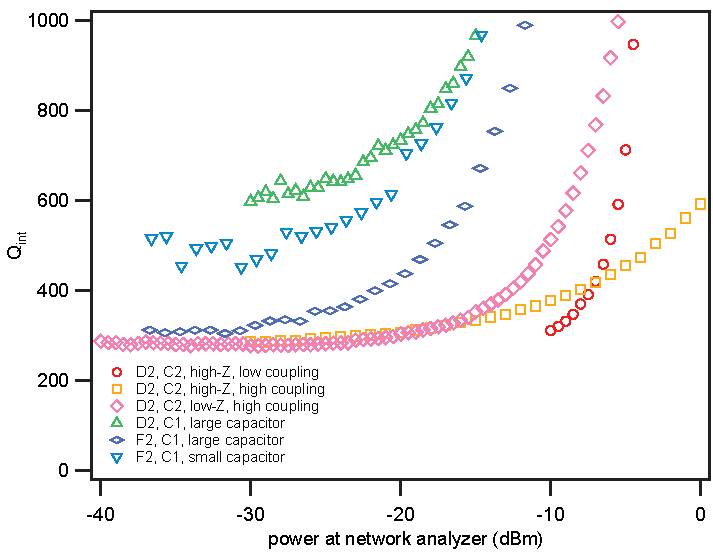
\includegraphics[width=4.75in]{twpa_exp/Qint}
\end{center}
\caption[Test resonator quality factor measurements]{Measured internal quality factors for six test resonators, three from the C1 layer and three from C2.  The traces have been offset on the power axis for clarity, to show the saturation in roughly the same regime.}
\label{fig:Qint}
\end{figure*}

If we assume that all of the internal loss in the resonator can be attributed to the dielectric loss in the capacitor, then the loss tangent of the material is just given by the inverse of $Q_i$.  The loss tangent of these types of deposited dielectrics tends to be relatively high, on the order of $10^{-3}$ to $10^{-2}$, while inductive losses and losses in the coupling capacitors should be very small compared to this.  As shown in Figure \ref{fig:Qint}, the C2 resonators have a fairly consistent $Q$ of about 300, while there is somewhat more scatter in C1 from 300 to 600 or so.  Because the transmission line capacitance is formed from C2, this is the most important loss in the system, corresponding to a loss tangent of about $3.3 \times 10^{-3}$.  Assuming no other losses in the line, the attenuation constant $\alpha$ of the transmission line in the small signal regime is then given by
\begin{equation}
\alpha = 8.686 \times \tan(\delta) \frac{\omega C Z_0}{2} = 2.03 \times 10^{-4} \frac{\mathrm{dB}}{\textrm{unit cell} \cdot \rm GHz}
\end{equation}
for $C = 45$ fF \cite{pozar1997microwave}.  Thus, a 2000 cell JTWPA should have a loss of about 1.6 dB at 4 GHz, and 4 dB at 10 GHz.

\section{Transmission measurements}

Because the JTWPA is a 2-port device and operates in a transmission mode, measuring the transmission through the device in a well-matched 50 $\Omega$ environment is the most fundamental and important measurement of device performance.  Measurements of reflection parameters are also of interest, though making this type of measurement in a well-calibrated manner in a cryogenic system is quite non-trivial and requires cryogenic calibration standards to make a meaningful measurement.  As such, I will focus on transmission measurements only.

\begin{figure*}
\begin{center}
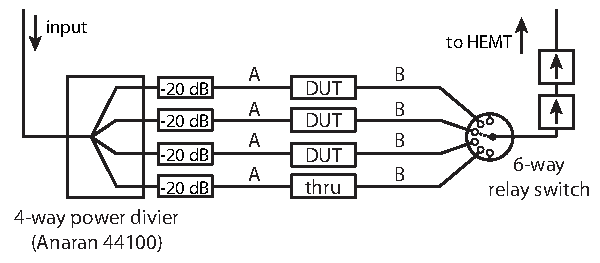
\includegraphics[width=4in]{twpa_exp/trans_meas}
\end{center}
\caption[Cryogenic calibrated transmission measurement setup]{Microwave circuit schematic for cryogenic calibrated transmission measurements, using passive input multiplexing and active output multiplexing.  Higher temperature stages not shown.}
\label{fig:trans_meas}
\end{figure*}

The cryogenic setup used for the majority of JTWPA measurements is shown schematically in Figure \ref{fig:trans_meas}.  The probe signals arrive at the cold stage of the dilution refrigerator and are passively split using a commercial 4-way 2-18 GHz power divider.  The relative power in each output is balanced to better than 0.1 dB.  A 20 dB attenuator is connected to the output of each port, ensuring the input to the device under test (DUT) is a well-matched 50 $\Omega$, and adding an effective 40 dB of isolation between each measurement arm.  With the 20 dB isolation of the splitter itself, this setup provides about 60 dB of total isolation between the measurement arms.  The output of each measurement arm is connected to one port of a 6-way microwave relay switch, which directs one of the outputs through two isolators to the HEMT amplifier, while presenting an open circuit to the other ports.  Two more DUTs could be added to this setup if the 4-way power divider is replaced by another 6-way relay switch, which was not available in the dilution refrigerator in which these experiments were conducted.

One of the splitter outputs is connected to a SMA female-female union in place of a DUT to represent the baseline calibration for the transmission measurement.  The cables used to connect the thru calibration and the DUTs to the power divider and the output multiplexing switch are nominally identical commercial flex cables made by Mini-Circuits, of lengths labeled A and B.  On one cooldown, one of the DUTs was replaced with another thru connector to check the balance of the different transmission arms; transmission through the two thru connections was indistinguishable at the 0.1 dB level.  The DUTs are normally housed in an aluminum enclosure with small slots through which SMA cables enter and leave.  The aluminum enclosure is contained within a single layer of Cryoperm magnetic shielding.  The DUTs are bolted to a copper plate which is thermalized to the cold stage of the dilution refrigerator using a thick copper wire protruding through the lid of the aluminum enclosure.  This enclosure is primarily a legacy from past experiments; because the JTWPAs are fabricated from Niobium, they become superconducting at around 9 K, much earlier in the cooldown process than when the aluminum enclosure becomes superconducting at about 1 K.  Because the JTWPA design does not involve any SQUID loops, the device behavior is not particularly sensitive to magnetic field fluctuations and so a high degree of magnetic shielding is not necessary.

\subsection{Length scaling of non-RPM devices}

\begin{figure*}
\begin{center}
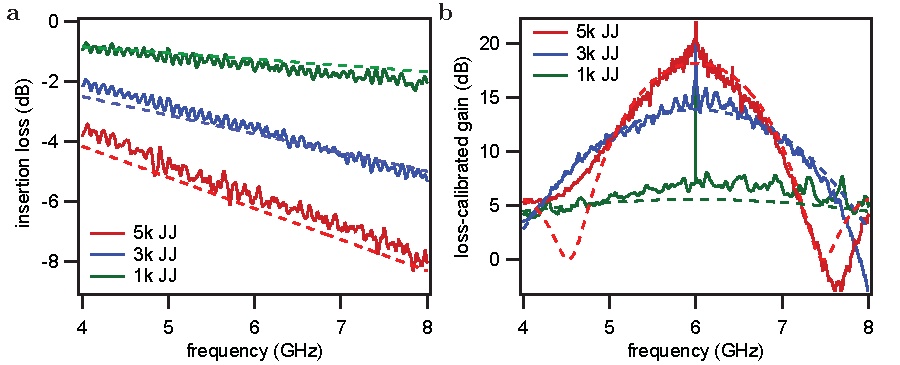
\includegraphics[width=6in]{twpa_exp/trad_dat}
\end{center}
\caption[Insertion loss and gain of non-RPM JTWPAs]{\textbf{a} Insertion loss for 1k, 3k, and 5k JJ devices, with theory predictions for a capacitor quality factor $Q_i = 291$.  \textbf{b} Measured gain profiles of 1k, 3k, and 5k JJ devices at identical pumping conditions ($\sim 0.75 I_0$), after subtracting the insertion loss measured in \textbf{a}, with theory overlays for the simple theory without loss.}
\label{fig:trad_dat}
\end{figure*}

To verify the theoretical prediction of quadratic scaling with device length for JTWPAs with no explicit modification to the dispersion relation, we measured three devices from Reticle A in the same cooldown, with lengths of 1k, 3k, and 5k unit cells\footnote{In reality, we measured many more of these types of devices, as they were the focus of the work before the addition of RPM loading structures.  For clarity I focus here on just three devices of the final generation.}.  The nominal device parameters are $I_0 = 3.1$ $\mu$A, $C_j = 55$ fF, and $C = 50$ fF, and the 1k, 3k, and 5k devices actually contained 1006, 3008, and 5022 junctions, respectively.

Data from these devices are shown in Figure \ref{fig:trad_dat}.  After calibrating the transmission using the thru, we measured the insertion loss of each device.  The measured insertion loss agrees well with the losses predicted by a simple model of capacitive dielectric losses with $\tan{\delta} = 0.0034$, in good agreement with the measured loss tangent of the material.  The gain of these devices is plotted with the insertion loss subtracted, to more directly show the quadratic scaling behavior with increasing length.  The agreement between the measured gain and the theory is quite reasonable, validating the simple prediction of quadratic scaling.

\subsection{Measurements of RPM loading structures}

For the remainder of this chapter I will focus on a very complete characterization performed on a single RPM-JTWPA device.  The device parameters are those listed in section \ref{s:twpa_fab}.  I will refer to this particular amplifier as Device A.

\begin{figure*}
\begin{center}
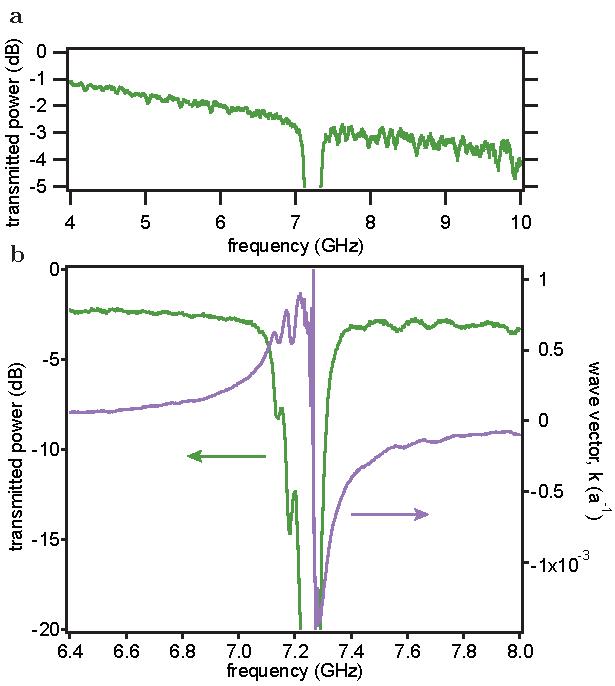
\includegraphics[width=4.1in]{twpa_exp/twpa_trans}
\end{center}
\caption[Transmitted power and wavevector shift]{\textbf{a} Broadband small-signal power transmission, with axis scaled to clearly show the dielectric insertion loss of 1 to 4 dB.  The transmission dip associated with the RPM resonators is visible just above 7 GHz. \textbf{b} Small-signal power transmission (green) and wavevector shift (purple) in the vicinity of the dispersion feature.  The large linear component of the wavevector has been subtracted to show just the shift associated with the dispersion feature.}
\label{fig:twpa_trans}
\end{figure*}

In the small-signal regime, an RPM-JTWPA should look identical to a JTWPA without loading structures except for the presence of a large transmission dip in the vicinity of the resonant frequency of the RPM resonators.  The small-signal transmission and wavevector shift for Device A is shown in Figure \ref{fig:twpa_trans}.  The insertion loss is comparable to that measured for non-RPM devices in Figure \ref{fig:trad_dat}.  The width of the RPM stop band is significantly larger than predicted for the ideal theory; this is due to some small frequency variation in the resonators, on the order of 1\%, which is sufficient to significantly broaden the stop-band and weaken the total wavevector shift.  This frequency heterogeneity is also responsible for the large ripples in transmission and wavevector on the low-frequency side of the dispersion feature.  Although the absolute magnitude of the wavevector shift is decreased compared to theory, it is still sufficient to partially phase match the four-wave mixing process.

\subsection{Gain with RPM}\label{s:gain_with_rpm}

\begin{figure*}
\begin{center}
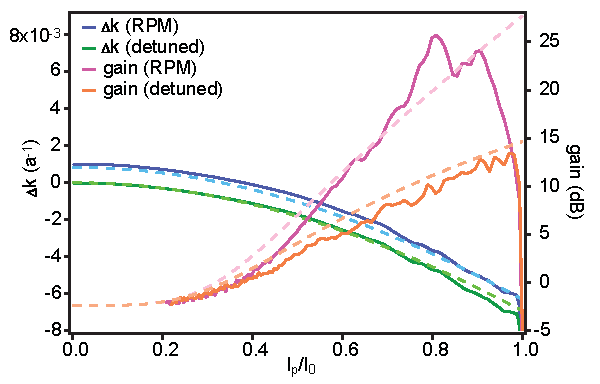
\includegraphics[width=4in]{twpa_exp/gain_and_dk}
\end{center}
\caption[Gain and phase mismatch comparison]{Total wavevector mismatch $\Delta k$ (left axis) and corresponding amplifier gain (right axis) for a signal at 6.584 GHz.  For the ``RPM'' traces, the pump was placed at 7.157 GHz, while the ``detuned'' traces have a pump at 6.5 GHz, far from the dispersion feature.  Theory predictions are overlaid on the data as dashed lines in complementary colors.  The total wavevector modification for the RPM case can be seen as the vertical offset on the left axis between the green and blue traces.}
\label{fig:gain_and_dk}
\end{figure*}

The effect of RPM on the device gain is shown in Figure \ref{fig:gain_and_dk}, where the wavevector mismatch and gain is plotted for a pump near the RPM feature and also for a pump far detuned.  The measured gain for the RPM case is about 10 dB larger than for the detuned case, even though the wavevector mismatch is still far from perfect at large pump powers.  The pump power axis is scaled using the sharp feature visible at the right of the plot, which roughly corresponds to the power at which the pump current exceeds the junction critical current.  This effect is used in all measurements to calibrate the pump power scale.

\begin{figure*}
\begin{center}
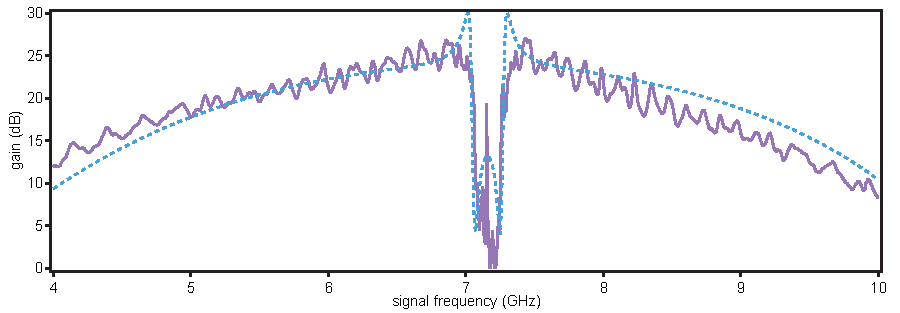
\includegraphics[width=6in]{twpa_exp/twpa_gain}
\end{center}
\caption[Ultra-broadband gain profile]{The gain profile measured with a pump at 7.157 GHz and a pump current of 91\% of the critical current.  A theory prediction for the measured device parameters, including the effects of loss for the signal and the pump, is overlaid as a blue dashed line.}
\label{fig:twpa_gain_exp}
\end{figure*}

The complete gain profile achieved with a pump at 7.157 GHz and $I_p / I_0 = 0.91$ is shown in Figure \ref{fig:twpa_gain_exp}.  Without exaggerating, the bandwidth achieved by Device A can be described as massive.  The gain exceeds 20 dB over a bandwidth of about 3 GHz, excluding the region near the dispersion feature, and exceeds 15 dB over an entire octave (from 4.5 to 9 GHz).  This is by far the largest bandwidth ever achieved in a Josephson parametric amplifier of any variety\footnote{This bandwidth has been superseded by a device from a subsequent seventh generation of JTWPAs, measured at LL.  That device achieved a bandwidth of 4.5 GHz with gain above 20 dB.}.  The gain profile shows a small ripple, on the order of $\pm 2$ dB, which we attribute to the impedance mismatch between the nonlinear JTWPA transmission line (which is about 42 $\Omega$ when pumped) and the linear 50 $\Omega$ feedlines to which it is coupled.  This leads to a small amount of reflection, with a period related to the electrical length of the JTWPA as discussed at the end of section \ref{s:twpa_param}.

The overlaid theory curve is based on the modified theory including the effect of finite pump and signal losses described in section \ref{s:twpa_loss_theory}.  The model parameters are determined from linear and nonlinear single-wave characterization. To obtain the wavevector, we measure the microwave transmission without a pump through the JTWPA. The real component of the wavevector is obtained from the phase of the transmitted field, $k' = (\phi(\omega)+\phi_0)/L$, and the magnitude of the transmission yields a frequency dependent imaginary wavevector, $k''=-\log(T)/(2L) \approx c_1 \omega + c_2^2 \omega^2$, where $c_1 = 2.0$ fs and $c_2 = 0.55$ fs,  away from the resonance. The signal and idler are attenuated more than the pump as the strong pump field partially saturates the frequency-dependent dielectric loss. The constant $\phi_0$ is determined from the zero-frequency limit of the wavevector. From a comparison of the experimentally-measured dispersion with the theoretical model for the wave-vector we obtain an estimate for the capacitance to ground of $C=45.6~\mathrm{fF}$. The junction parameters are obtained from electrical characterization as detailed in section \ref{s:twpa_fab}. We model the effect of inhomogeneity in the dispersion loading resonators as a single resonant mode with a loaded Q selected to best match the width of the observed transmission dip.

\section{Noise measurements}

A high-gain, broadband amplifier is only useful if the amplifier operation is quiet.  For the JTWPA, the goal is to saturate the ideal quantum lower bound on added noise, as discussed in chapter \ref{c:paramps}.  To conclusively demonstrate noise near the quantum limit, precision measurements must be made to ensure that the systematic errors are fractionally small compared to the measured value.  A noise measurement that concludes that the amplifier is quantum-limited \textit{plus or minus the quantum limit} is both uninteresting and unphysical.

\subsection{System noise temperature extraction}

The fundamental challenge for making precise cryogenic noise measurements is the need for a calibrated power reference at the cold stage of the dilution refrigerator.  Injecting a signal which is calibrated at room temperature into the system is insufficient, as the insertion loss between room temperature and the cold stage cannot be directly measured when the system is cold.  Measuring the total round-trip transmission doesn't help either, as the gain of the HEMT amplifier and the insertion loss back up to room temperature is equally unknown.  Thus, we must find some physical process which produces a calibrated reference power at the cold stage, ideally at a relevant reference plane for characterizing an amplifier.

The two most commonly-used physical processes are the Johnson noise of a variable-temperature matched load \cite{Fernandez1998} and the shot noise of a tunnel junction \cite{Spietz2003}.  Although both of these techniques provide a precisely-calibrated broadband noise level, they suffer from the same general class of drawbacks: each technique requires an intermediate microwave network between the calibrated source and the remainder of the microwave measurement chain which is unrelated to the general measurement setups in which the amplifiers will be used.  For the variable-temperature load, an intermediate piece of coaxial cable is needed to permit the temperature of the load to be varied independently of the rest of the measurement chain.  Because thermal conductivity in a metal is provided by the electrical conductivity at dilution refrigerator temperatures, this typically implies that this cable is made of a lossy material such as stainless steel, introducing an unknown insertion loss on the order of 1-2 dB.  For the shot noise tunnel junction source, a bias tee is needed to inject the DC voltage to bias the tunnel junction, introducing an unknown insertion loss on the order of 1-2 dB.  As a result of these unknown losses, the total system noise temperature reported using these techniques typically comes with systematic uncertainty of the same order, preventing a precise determination of the system noise \cite{Castellanos-Beltran2008,Mutus2014}.

\subsection{Circuit QED power calibration}

\begin{figure*}
\begin{center}
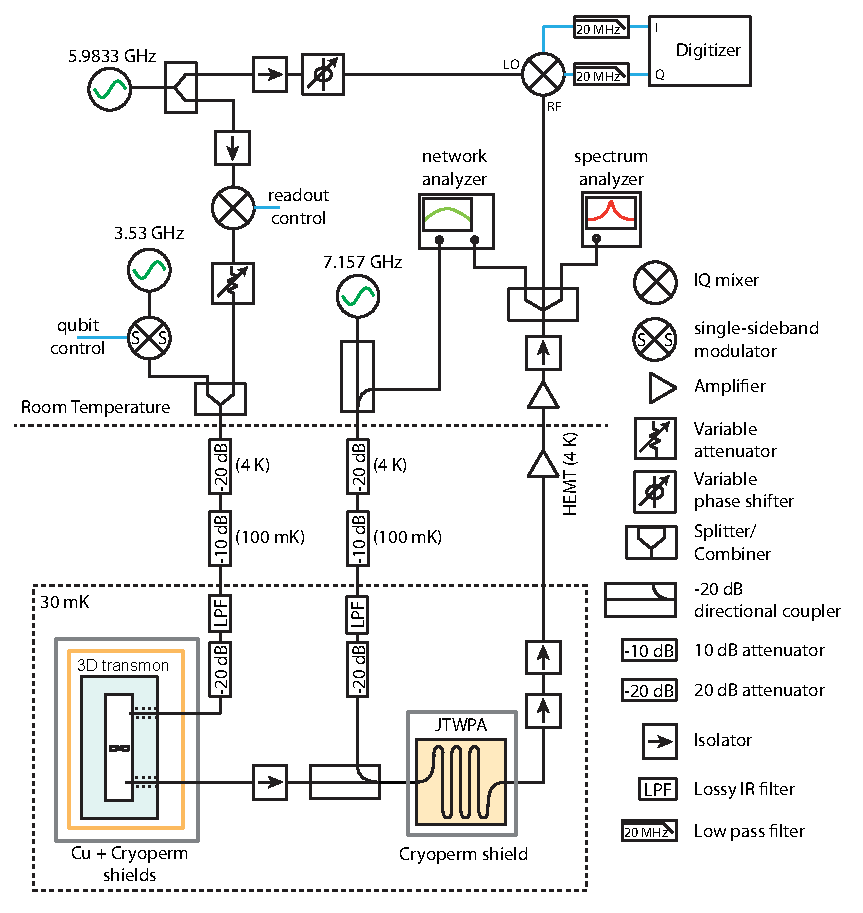
\includegraphics[width=5in]{twpa_exp/noise_schem.pdf}
\end{center}
\caption[Microwave measurement schematic for system noise measurement]{Schematic diagram of microwave measurement setup for system noise temperature measurements.  Gain measurements are made \textit{in situ} by injecting an additional measurement signal from a vector network analyzer through a directional coupler on the pump line at room temperature.}
\label{fig:noise_schem}
\end{figure*}

Instead of these calibrated noise reference techniques, we utilize the AC Stark shift of a cQED system to precisely calibrate the photon number occupation of the cavity.  A schematic of the full microwave setup used in these experiments is shown in Fig \ref{fig:noise_schem}.  By independently measuring the cavity frequency $\omega_r$ and output coupling rate $\kappa$, the output power is then precisely determined as $P = \kappa \hbar \omega_r \bar{n}$.  This is the same technique as is used to determine $\eta_\mathrm{det}$ in section \ref{s:det_meas_eta}.  Because we use a cQED system as the source of the power calibration, there is no additional uncertainty in determining the relevant system noise temperature delivered by a particular parametric amplifier in a real experimental context, as the experiment itself serves as the reference plane.  The primary downside of this technique compared to a calibrated noise reference is the fundamentally narrowband nature of the cavity power calibration, so we will only be able to extract the system noise at the cavity frequency.

The cQED system used here was again a single-junction 3D transmon.  The qubit had a transition frequency $\omega_{qb}/2 \pi = 3.58$ GHz, measured precisely with Ramsey oscillations, and $T_1 = 22$ $\mu$s.   The cavity parameters are directly measured by fitting the cavity transmission spectrum to a Lorentzian function, as shown in Figure \ref{fig:kappa}, resulting in $\omega_r / 2 \pi = 5.984$ GHz and $\kappa / 2 \pi = 18.5$ MHz.

\begin{figure*}
\begin{center}
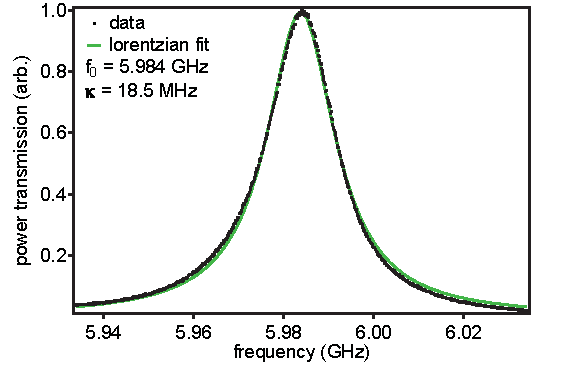
\includegraphics[width=3.75in]{twpa_exp/kappa}
\end{center}
\caption[Lorentzian fit of cavity resonance]{Lorentzian fit to cavity resonance.  The measured cavity transmission spectrum deviates slightly from a perfect Lorentzian profile; we attribute this variation to transmission ripple in the microwave measurement chain, which is generally smooth but becomes significant on the order of 30 MHz.}
\label{fig:kappa}
\end{figure*}

We calibrate the dispersive shift $\chi$ using two techniques.  First, we utilize the same AC Stark shift and measurement dephasing technique described in section \ref{s:chi_cal}, though in this round of measurements we took a significantly larger quantity of data to reduce the noise and improve our estimate of $\chi$ to the 1\% level.  The extracted AC Stark shift and dephasing rates versus measurement power are shown in Figure \ref{fig:gamma_and_stark}a along with the resulting calibration between input power and $\bar{n}$ (Figure \ref{fig:gamma_and_stark}b); from the fits, we extract $\chi = 584 \pm 5$ kHz.

As an independent check on this result, we directly measure the phase shift in the transmitted microwave signal for different qubit states.  This data is shown in Figure \ref{fig:gamma_and_stark}c.  We use postselection to purify an ensemble of qubit states in $|0\rangle$ and $|1\rangle$ (see section \ref{s:weak_meas} for more details).  We then integrate an intermediate measurement period and plot the resulting points in the IQ plane.  We measure an angular separation $\Delta \theta = 7.3$ degrees, implying a value for the ratio $\chi / \kappa = \frac{1}{2} \tan{(\Delta \theta/2)} = 3.18 \times 10^{-2}$.  From the direct measurement of $\kappa$ and the value for $\chi$ extracted using the AC Stark shift measurement, we find $\chi / \kappa = (3.16 \pm 0.03) \times 10^{-2}$, in excellent agreement.  There is a slight 1\% asymmetry in the length of the two coherent state vectors, likely due to the measurement frequency not being exactly at the midpoint between the cavity frequencies associated with the first two qubit states.

This direct measurement of $\Delta \theta$ requires precisely calibrating the demodulation setup.  In general, the three first-order imperfections in the demodulation setup are unequal gains and DC offsets in the low-frequency signal path for the I and Q outputs, as well as skew in the axes represented by I and Q (implying some mixing of one axis into the other).  All of these effects can be measured simultaneously by injecting a signal which is slightly detuned from the local oscillator, producing oscillations in I and Q at the detuning frequency.  By fitting these oscillations to sine and cosine and extracting the offset, amplitude, and phase shift, we can calculate a transformation which removes all of these effects to first order. 

\begin{figure*}
\begin{center}
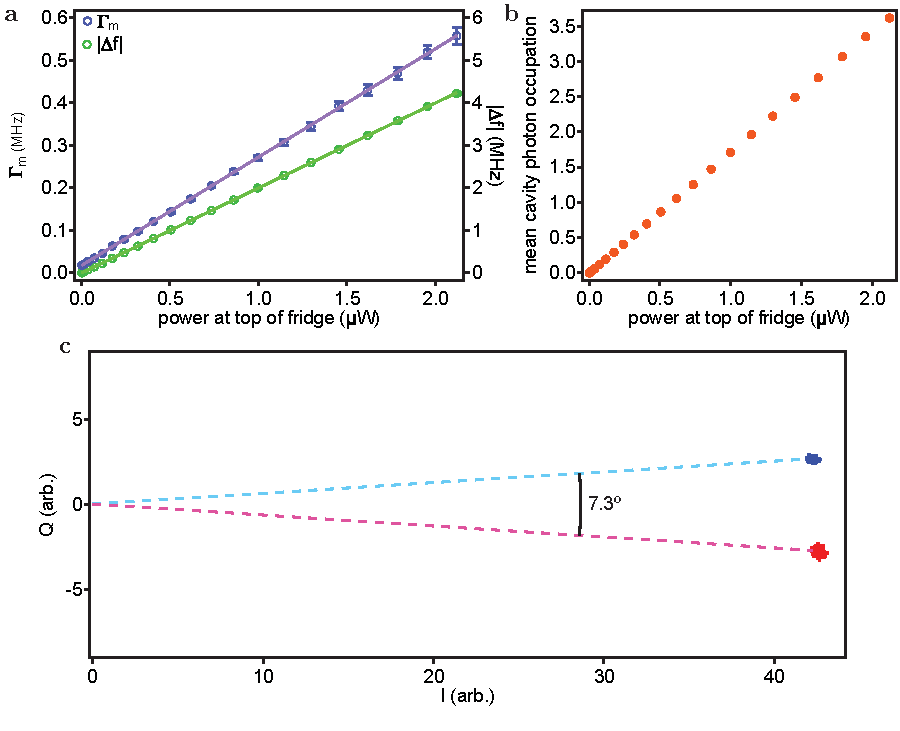
\includegraphics[width=6in]{twpa_exp/gamma_and_stark}
\end{center}
\caption[$\chi$ calibration, two ways]{\textbf{a} Linear fits to measured dephasing rate and AC Stark shift versus weak measurement power.
\textbf{b} Calculated mean cavity photon occupation from calibrated value of $\chi$ and the measured AC stark shift. \textbf{c} Purified qubit readout histograms.  We independently estimate the ratio $\chi / \kappa$ by measuring the phase shift in the transmitted microwave signal for ensembles of purified qubit states, finding a phase shift between the ground state and excited state histograms of 7.3 degrees.}
\label{fig:gamma_and_stark}
\end{figure*}

\subsection{Noise power}\label{s:noise_pow}

With the photon number calibration in hand, measuring the system noise temperature referred to the cavity output is as simple as measuring the ouput noise spectrum of the microwave measurement chain while simultaneously injecting a calibrated signal power.  In practice, we excite the cavity with a calibrated $\bar{n}$ and measure the resulting power at the output using a spectrum analyzer.  We then turn the cavity excitation off, and inject a tone directly down the JTWPA pump line, bypassing the cavity, and adjust the generator power until we measure the same power at the spectrum analyzer.  This procedure calibrates this signal power to the same plane as the photon number calibration, but avoids any extra noise associated with thermally-induced qubit transitions or small qubit-cavity nonlinearities at high drive powers from contaminating the amplifier measurement.

\begin{figure*}
\begin{center}
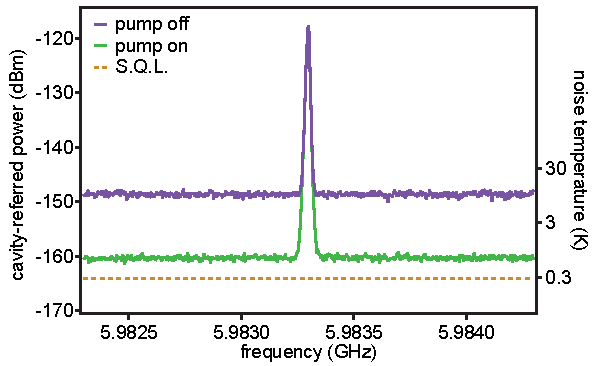
\includegraphics[width=4in]{twpa_exp/snr_trace}
\end{center}
\caption[Calibrated output noise spectra]{Calibrated output noise spectra.  The spectrum taken with the pump on is referred to back to the input by subtracting the measured amplifier gain.}
\label{fig:snr_trace}
\end{figure*}

Noise power spectra taken of the output microwave field in the vicinity of the cavity frequency are shown in Figure \ref{fig:snr_trace}.  The coherent tone corresponding to a mean cavity occupation $\bar{n} = 3.62 \pm 0.04$ allows us to calibrate a cavity-output-referred power axis (left) as well as a system noise temperature axis using Boltzmann's constant and the 10 kHz measurement bandwidth (right).  With the JTWPA pump off we extract a system noise of $9.01 \pm 0.23$ K.  This is a very reasonable number; the HEMT amplifier is manufactured by Low Noise Factory (model LNC4-8A) and has a specified noise temperature of 3 K.  If the HEMT is meeting this specification, then a 9 K system noise implies an insertion loss of 4.8 dB between the cavity and the HEMT, including 2.0 dB of loss in the JTWPA.  Considering the passive microwave network in this portion of the measurement chain contains a directional coupler and three isolators, an insertion loss of 2.8 dB is very reasonable (a typical rule of thumb is 0.5 to 1 dB per component).  We turn the pump on and measure a signal gain of 21.6 dB; we refer the resulting noise level to the cavity output by subtracting this gain from the measured trace, permitting a direct comparison of noise temperature.  We measure a system noise of $602 \pm 15$ mK, or about twice the one-photon quantum limit, equivalent to a quantum measurement efficiency $\eta = 0.48 \pm 0.016$.

\subsection{Weak measurement}\label{s:weak_meas}

We make an independent assessment of the quantum efficiency using the results for dephasing in a circuit QED measurement \cite{Boissonneault2009}.  In the limit relevant to weak measurement, the dephasing rate is given by $\Gamma_m = 8 \chi^2 \bar{n} / \kappa$.  The rate of qubit state information collection is related to the signal-to-noise ratio (SNR) of integrated readout histograms as $\Gamma_m' = (\textrm{SNR})^2 / 8 \tau$ where $\tau$ is the measurement integration time \cite{Korotkov2001}.  The quantum efficiency is the ratio of these two quantities, $\eta = \Gamma_m' / \Gamma_m$, which saturates to 1 when the dephasing rate and the rate of information collection are equal.

\begin{figure*}
\begin{center}
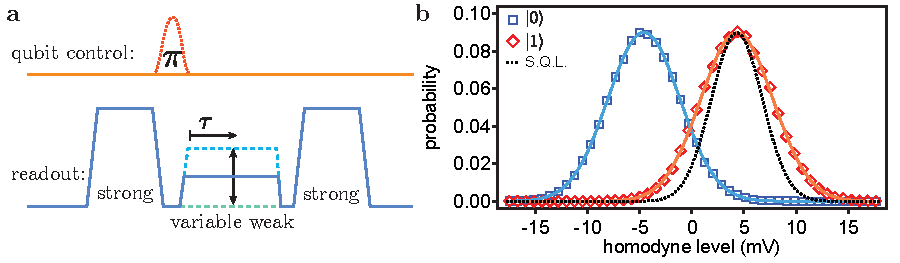
\includegraphics[width=6in]{twpa_exp/weak_meas}
\end{center}
\caption[Weak measurement extraction of $\eta$]{\textbf{a} Qubit and measurement pulse sequence.  \textbf{b} Example weak measurement histograms with $\bar{n} = 3.62$ and $\tau = 1$ $\mu$s with gaussian fits.  The black dashed line illustrates the histogram width expected for a fully quantum-limited measurement.}
\label{fig:weak_meas}
\end{figure*}

The control sequence for this measurement is shown in Figure \ref{fig:snr_trace}a.  We use heralding to post-select a pure ground state ensemble \cite{fluxqb}.  We prepare half of the ensemble in $|1\rangle$ by applying a $\pi$-pulse and leave the other half in $|0\rangle$, followed by a weak measurement of variable amplitude.  A final strong measurement allows the use of post-selection to eliminate records that underwent an undesired state transition.  In this manner, we create very pure ensembles; the only non-ideal events which can contaminate these ensembles are experimental records which underwent two or more spontaneous state transitions during the weak measurement period.  With the long $T_1$ time of this qubit, this type of event is fairly rare\footnote{We can crudely estimate an upper bound on this effect in the following manner.  The total time between the strong measurements $\tau_m$ is less than 5 $\mu$s, and the probability of finding the qubit in the excited state in thermal equilibrium $P_{\ket{1},\mathrm{therm}}$ is smaller than 5\%.  If we assume the thermalization time scale is the same as $T_1$, then the probability of a qubit starting in the excited state, decaying due to $T_1$, and then being thermally re-excited is smaller than $P_{\ket{1},\mathrm{therm}} [ 1 - \exp{(-\tau_m / T_1)}]^2  = 0.002$.  The fact that these events can only have one physical time-ordering of course further suppresses this probability.}.

All of the weak measurement period is digitized, allowing for the integration time to be chosen during data analysis.  We integrate the weak measurement for various times in the range 1 to 4.6 $\mu$s and histogram the results.  One set of these histograms is shown in Figure \ref{fig:weak_meas}b.  We fit the histograms for the $|0\rangle$ and $|1\rangle$ sub-ensembles to Gaussian functions and extract the SNR.  We repeat this experiment for a range $\bar{n}$ from 0.3 to 3.6, extracting a mean quantum efficiency $\eta = 0.49 \pm 0.01$, in excellent agreement with the result obtained from the noise power method.

\subsection{Quantum efficiency analysis}

The directly measured noise quantity in these experiments is the quantum efficiency of the entire microwave measurement chain, $\eta$, referred to the plane coincident with the output of the 3D cavity.  This single number involves contributions from several sources that all conspire to reduce the quantum efficiency of the measurement chain from unity.  We identify four different components to the measured value: insertion loss between the cavity and JTWPA ($\eta_L$), the insertion loss of the JTWPA itself ($\eta_D$), the finite size of the HEMT noise compared to the amplified quantum noise at the output of the JTWPA ($\eta_H$), and finally an additional factor due to possible unknown factors intrinsic to the JTWPA itself ($\eta_J$).

We measure the insertion loss of the intermediate microwave network between the cavity and the JTWPA in a separate measurement at 77 K.  We find an insertion loss of 1.6 dB at 5.9833 GHz, equivalent to $\eta_L = 0.69$.  We can estimate $\eta_D$ using the theory developed in section \ref{s:twpa_dist_loss}.  From Figure \ref{fig:twpa_trans}, we extract a small-signal insertion loss of 2.0 dB at 5.9833 GHz.  If we attribute all of this loss to the dielectric loss in the capacitance to ground in each unit cell, then the attenuation per unit cell is $A_i = 9.8 \times 10^{-4}$ dB.  At the operating point used for the weak measurement calibration of $\eta$, the JTWPA provided 21.6 dB of gain.  In the simple approximation of purely exponential gain with length, each unit cell delivers $1.06 \times 10^{-2}$ dB of gain.  From \eqref{eq:eta_D}, we predict an input-referred noise of 1.1 quanta, or a quantum efficiency $\eta = 0.9$.  Utilizing the full gain profile in length predicted from theory provides a very small correction to this number, a further reduction in $\eta$ on the order of 0.001.  This result suggests that the use of a relatively lossy SiO$_2$ dielectric is not a dominant effect in setting the noise temperature of the amplifier.  With only a modest reduction in dielectric loss tangent, the contribution of the distributed loss in the amplifier to the quantum efficiency can be further reduced to the few-percent level.

If the JTWPA were fully quantum-limited, the output noise at the input to the HEMT would be 41.5 K, implying the 3 K HEMT noise is not completely negligible compared to the amplified quantum noise.  From these values we calculate $\eta_H = 0.93$.  Combining these results and solving for the unknown factor gives $\eta_J = 0.85$, implying that the parametric process in the JTWPA is operating with a high quantum efficiency.  Although $\eta_D$ is not fundamental to the JTWPA and can be reduced in future devices by using a lower-loss dielectric, we consider it to be part of the intrinsic quantum efficiency of this device. Thus, we calculate the quantum efficiency of Device A as $\eta_D \eta_J = 0.76$.  These values are realistically just estimates and could easily have unaccounted-for systematic errors of 10-20\%.

\section{Projective qubit readout}

Because one of the motivating applications of the JTWPA is the simultaneous readout of multiple superconducting qubits, evaluating the performance of the amplifier in the context of projective qubit readout is important.  From a quantitative standpoint, the projective measurement performance of the amplifier only depends on the input compression power and the measurement efficiency, as these two quantities determine how well qubit readout histograms can be separated.  For reading out more than one qubit, the amplifier bandwidth is also important, as each qubit will typically have its own readout resonator, and to ensure a clean readout of each qubit the detuning between cavity frequencies should be at least several cavity linewidths.  The very large bandwidth of the JTWPA handily satisfies this condition for typical cQED parameters; with $\kappa = 10$ MHz and a $5\kappa$ detuning, about 30 readout resonators could fit into one gain sideband.

\subsection{Input compression power}

\begin{figure*}
\begin{center}
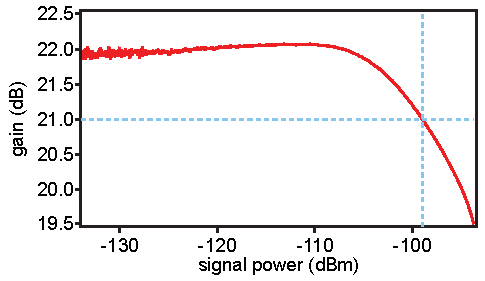
\includegraphics[width=3.24in]{twpa_exp/dr}
\end{center}
\caption[JTWPA input compression]{Measured input power gain compression curve, showing $P_{1\mathrm{dB}} = -99$ dBm.}
\label{fig:dr}
\end{figure*}

From the same signal power calibration used in section \ref{s:noise_pow}, we can measure the gain of the amplifier as a function of the input signal power.  This measurement is shown in Figure \ref{fig:dr}, with 1 dB gain compression occurring with an input signal of -99 dBm.  This value is about 10 dB larger than demonstrated in any JPA with comparable gain \cite{Eichler2014a,Mutus2014}.

\subsection{Single-qubit readout and extrapolation}\label{s:twpa_proj_meas}

Lacking a multi-qubit platform, we instead use a single 3D transmon to benchmark the projective readout performance of the JTWPA.  Realizing a good projective measurement requires a cQED system optimized in a different regime than the weak measurement regime used for the noise calibrations; namely, the dispersive shift $2\chi$ should be of the same order as $\kappa$, the cavity linewidth\footnote{Technically speaking there is a global optimum at $2\chi = \kappa$, but this is not stringently required for good projective readout.}.  As such, we substitute another qubit into the cavity with a smaller qubit-cavity detuning $\Delta$, and decrease the output coupling rate, both of which enhance the ratio $\chi/\kappa$.  The values achieved in the experiment were $\chi/2\pi = 2.2$ MHz and $\kappa/2\pi = 8.7$ MHz.  The qubit had a relatively short relaxation time $T_1 = 6$ $\mu$s.

\begin{figure*}
\begin{center}
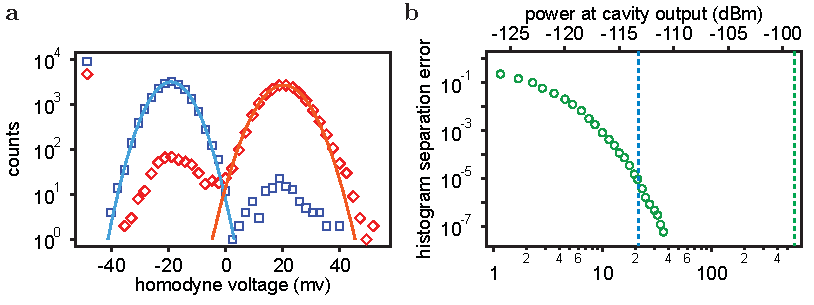
\includegraphics[width=5.42in]{twpa_exp/proj_meas}
\end{center}
\caption[Projective qubit measurement with JTWPA]{\textbf{a} Optimized projective readout histograms.  The intrinsic overlap of the histograms contributes less than $10^{-5}$ of the total error.  \textbf{b} Histogram separation error for 100 ns integration window.  The measurement power required to achieve a histogram separation error below $10^{-5}$ (dashed blue line) is 14 dB below the measured 1 dB compression power of the JTWPA (dashed green line).}
\label{fig:proj_meas}
\end{figure*}

The control sequence for projective readout is the same as in Figure \ref{fig:weak_meas}a except for the absence of the weak measurement.  Using $\bar{n} = 23.3$ and a 100 ns integration window, we measure the well-separated readout histograms shown in Figure \ref{fig:proj_meas}a.  We extract a raw measurement fidelity $F = 1 - P_{1|0} - P_{0|1} = 0.967$ where $P_{a|b}$ is the probability of identifying the qubit state as $|a\rangle$ when it was prepared as $|b\rangle$.  The error is dominated by relaxation of the qubit and spurious excitation between the heralding readout and the final readout, contributing 0.026 and 0.007, respectively.  Based on Gaussian fits to the state histograms, the intrinsic overlap contributes about $10^{-5}$ of the total measurement error.  The readout error due to this histogram overlap (associated with the quantum efficiency) is plotted versus readout power (and $\bar{n}$) in Figure. \ref{fig:proj_meas}b.  The readout power needed to achieve a $10^{-5}$ error level is 14 dB below the 1 dB compression power of the JTWPA, implying that over 20 qubits could be simultaneously read out without a degradation in performance.
`






